%
% gamma.tex -- Abschnitt über die Gamma-funktion
%
% (c) 2021 Prof Dr Andreas Müller, OST Ostschweizer Fachhochschule
%
\section{Die Gamma-Funktion
\label{buch:rekursion:section:gamma}}
Die Fakultät $x!$ kann rekursiv durch 
\[
	x! = x\cdot (x-1)! \qquad\text{und}\qquad 0!=1
\]
für alle natürlichen Zahlen $x\in\mathbb{N}$ definiert werden.
Äquivalent damit ist eine Funktion 
\begin{equation}
\Gamma(x+1) = x\Gamma(x)
\qquad\text{und}\qquad 
\Gamma(1)=1.
\label{buch:rekursion:eqn:gammadef}
\end{equation}
Kann man eine reelle oder komplexe Funktion finden, die die
Funktionalgleichung~\eqref{buch:rekursion:eqn:gammadef}
erfüllt und damit die Fakultät auf beliebige Argumente ausdehnt?

\subsection{Integralformel für die Gamma-Funktion}
Euler hat die folgende Integraldefinition der Gamma-Funktion gegeben.

\begin{definition}
\label{buch:rekursion:def:gamma}
Die Gamma-Funktion ist die Funktion 
\[
\Gamma
\colon
\{z\in\mathbb{C} \mid \operatorname{Re}z>0\}
\to \mathbb{C}
:
z
\mapsto
\Gamma(z) = \int_0^\infty t^{x-1}e^{-t}\,dt
\]
\end{definition}

Man beachte, dass das Integral für $x=0$ nicht definiert ist, eine
Potenzreihenentwicklung um einen Punkt $x_0$ auf der positiven reellen
Achse kann also höchstens den Konvergenzradius $\varrho=|x_0|$ haben.

\begin{figure}
\centering
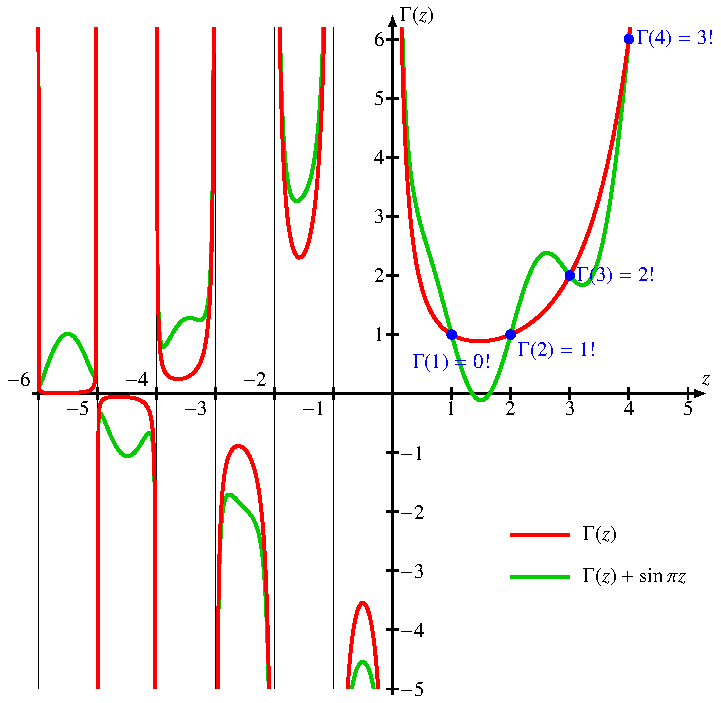
\includegraphics{chapters/040-rekursion/images/gammaplot.pdf}
\caption{Graph der Gamma-Funktion $z\mapsto\Gamma(z)$ und der alternativen
Funktion $\Gamma(z)+\sin(\pi z)$, die für ganzzahlige Argumente ebenfalls
die Werte der Fakultät annimmt.
\label{buch:rekursion:fig:gamma}}
\end{figure}

\subsubsection{Alternative Lösungen}
Die Funktion $\Gamma(z)$ ist nicht die einzige Funktion, die natürlichen
Zahlen die Werte $\Gamma(n+1) = n!$ der Fakultät annimmt.
Indem man eine beliebige Funktion $f(z)$ addiert, die auf alle
natürlichen Zahlen verschwindet, also $f(n)=0$ für $n\in\mathbb{N}$,
erhält man eine weitere Funktion, die auf natürlichen Zahlen
die Werte der Fakultät annimmt.
Ein Beispiel einer solchen Funktion ist
\begin{equation}
z\mapsto f(z)=\Gamma(z) + \sin \pi z,
\label{buch:rekursion:eqn:gammaalternative}
\end{equation}
die Funktion $f(z)=\sin\pi z$ verschwindet sogar auf allen ganzen
Zahlen.

In Abbildung~\ref{buch:rekursion:fig:gamma} ist die Gamma-Funktion
in rot geplotet, die Funktion~\eqref{buch:rekursion:eqn:gammaalternative}
in grün.
Die Punkte $(n,(n-1)!)$ sind in blau bezeichnet, sie sind beiden Graphen
gemeinsam.

\subsubsection{Pol erster Ordnung bei $z=0$}
Wir haben zu prüfen, dass sowohl der Wert $\Gamma(1)$ korrekt ist als
auch die Rekursionsformel~\eqref{buch:rekursion:eqn:gammadef} gilt.
Der Wert für $z=1$ ist
\begin{align*}
\Gamma(1)
&=
\int_0^\infty t^{1-1}e^{-t}\,dt
=
\left[ -e^{-t} \right]_0^\infty
=
1.
\end{align*}
Für die Rekursionsformel kann mit Hilfe von partieller Integration
bekommen:
\begin{align*}
\Gamma(z+1)
&=
\int_0^\infty t^{z+1-1}e^{-t}\,dt
=
\biggl[-t^{z}e^{-t}\biggr]_0^\infty
+
\int_0^\infty z t^{z-1}e^{-t}\,dt
\\
&=
z
\int_0^\infty
t^{z-1}e^{-t}\,dt
=
z \Gamma(z).
\end{align*}

Für $0<z<\varepsilon$ für eine $\varepsilon >0$ folgt aus der 
Funktionalgleichung
\[
\Gamma(z) = \frac{\Gamma(1+z)}{z}.
\]
Da $\Gamma(1)=1$ ist und $\Gamma$ eine in einer
Umgebung von $1$ stetige Funktion ist, kann sie in der Form
\(
\Gamma(1+z)=\Gamma(1) + zf(z)
\)
schreiben, wobei  $f(z)$ eine differenzierbare Funktion ist mit
$f'(1)=\Gamma'(1)$.
Daraus ergibt sich für $\Gamma(z)$ der Ausdruck
\[
\Gamma(z) = \frac{\Gamma(1)}{z} + f(z) = \frac{1}{z} + f(z).
\]
Die Gamma-Funktion hat daher and er Stelle $z=0$ einen Pol erster Ordnung.

\subsubsection{Ausdehnung auf $\operatorname{Re}z<0$}
Die Integralformel konvergiert nicht für $\operatorname{Re}z\le 0$.
Durch analytische Fortsetzung, wie sie im
Abschnitt~\ref{buch:funktionentheorie:section:fortsetzung}
beschrieben wird, kann die Funktion auf ganz $\mathbb{C}$ ausgedehnt
werden, mit Ausnahme einzelner Pole.
Die Funktionalgleichung gilt natürlich für alle $z\in\mathbb{C}$,
für die $\Gamma(z)$ definiert ist.
In einer Umgebung von $z=-n$ gilt
\[
\Gamma(z)
=
\frac{\Gamma(z+1)}{z}
=
\frac{\Gamma(z+2)}{z(z+1)}
=
\frac{\Gamma(z+3)}{z(z+1)(z+2)}
=
\dots
=
\frac{\Gamma(z+n)}{z(z+1)(z+2)\cdots(z+n-1)}
\]
Keiner der Faktoren im Nenner verschwindet in der Nähe von $z=-n$, der
Zähler hat aber einen Pol erster Ordnung an dieser Stelle.
Daher hat auch der Quotient einen Pol erster Ordnung.
Abbildung~\ref{buch:rekursion:fig:gamma} zeigt die Pole bei den
nicht negativen ganzen Zahlen.





